\documentclass[final]{beamer} % beamer 3.10: do NOT use option hyperref={pdfpagelabels=false} !
  %\documentclass[final,hyperref={pdfpagelabels=false}]{beamer} % beamer 3.07: get rid of beamer warnings
  \mode<presentation> { \usetheme{UFPoster} }
  \usepackage[english]{babel}
  \usepackage[latin1]{inputenc}
  \usepackage{amsmath,amsthm, amssymb, latexsym}
  \usefonttheme[onlymath]{serif}
  \boldmath
  \usepackage[orientation=portrait,size=a0,scale=1.1,debug]{beamerposter}                       % e.g. for DIN-A0 poster
  \title[Epi. on Emp. Nets]{Epidemics on Dynamic,\\ Empirical Networks}
  \author[Pearson \& Hladish]{Carl A.~B.~Pearson \&\ Thomas J.~Hladish}
  \institute[EPI-UF]{Emerging Pathogens Institute, University of Florida}
  \date{\today}
  \newcommand{\spaceProp}{0.02}
  \newcommand{\spacer}{\begin{column}{\spaceProp\paperwidth}\end{column}}
  
  \newenvironment{oneCol}{\begin{column}[t]{0.225\paperwidth}}{\end{column}}
  \newenvironment{threeCol}{\begin{column}[t]{0.715\paperwidth}}{\end{column}}
  
\usepackage{Sweave}
\begin{document}


\input{poster-concordance}
  \begin{frame}{}
    \begin{columns}[t]
    \spacer{}
    \begin{oneCol}
    \begin{block}{Introduction}
Contact networks are \textbf{intrinsically temporal}, but often analyzed as \textbf{time-aggregated} to simplify analysis and simulation.  Simulation on empirical networks, however, may skip this aggregation with minimal additional complexity.

We consider such simulation on $\mathbf{P\approx 2\times 10^6}$\textbf{ nodes}, interacting via $\mathbf{N\approx 2\times 10^6}$\textbf{ edges}, \textbf{over 5-years} of geo-temporal co-location data, derived from municipal WiFi access at businesses.  We start with a \textbf{review of network measures for different aggregation windows} on that data, and \textbf{conclude comparing simulated infections on these dynamic networks}.
%     \begin{block}{\large Fontsizes}
%       \centering
%       {\tiny tiny}\par
%       {\scriptsize scriptsize}\par
%       {\footnotesize footnotesize}\par
%       {\normalsize normalsize}\par
%       {\large large}\par
%       {\Large Large}\par
%       {\LARGE LARGE}\par
%       {\veryHuge veryHuge}\par
%       {\VeryHuge VeryHuge}\par
    \end{block}
    \begin{block}{Materials}
Network analysis and epidemic simulation used EpiFire\cite{hladish2012epifire}.  Visualization and poster prepared with Rweave, source @ \href{https://github.com/pearsonca/epidemics4-talk}{github.com/pearsonca/epidemics4-talk}.
    \end{block}
    \begin{block}{Methods}
Network measures computed in the standard way, after edges are determined on a per-time-period basis.  An edge exists between individuals if their access periods at a location overlap during a time period.

The epidemic is simulated given three parameters:\begin{itemize}
\item transmission probability along a contact per simulation time, $\rho$,
\item latent period, $\lambda_L$, and
\item infectious period, $\lambda_I$
\end{itemize}

We selected the $\lambda$s from literature estimates for influenza.  We fit $\rho$ for each binning scale to reproduce mean final size literature estimates for influenza.  The simulation proceeds as typical for a static contact network, however as time passes one of the binning boundaries, edges are added and removed accordingly.
    \end{block}
    \begin{block}{Mathematical Section}
Probably not relevant.  Maybe restate the network measures?  Diagram SIR flow?
    \end{block}
    \begin{block}{Conclusion}
The aggregation of empirical observations has important implications for simulation results.
    \end{block}
    \begin{block}{References}
      \nocite{*} % Insert publications even if they are not cited in the poster
      \small{\bibliographystyle{unsrt}
      \bibliography{biblio}\vspace{0.75in}}
    \end{block}
    \end{oneCol}
    \spacer{}
    \begin{threeCol}
    \begin{block}{Results}
    \begin{columns}
    \begin{oneCol}
        \begin{figure}
    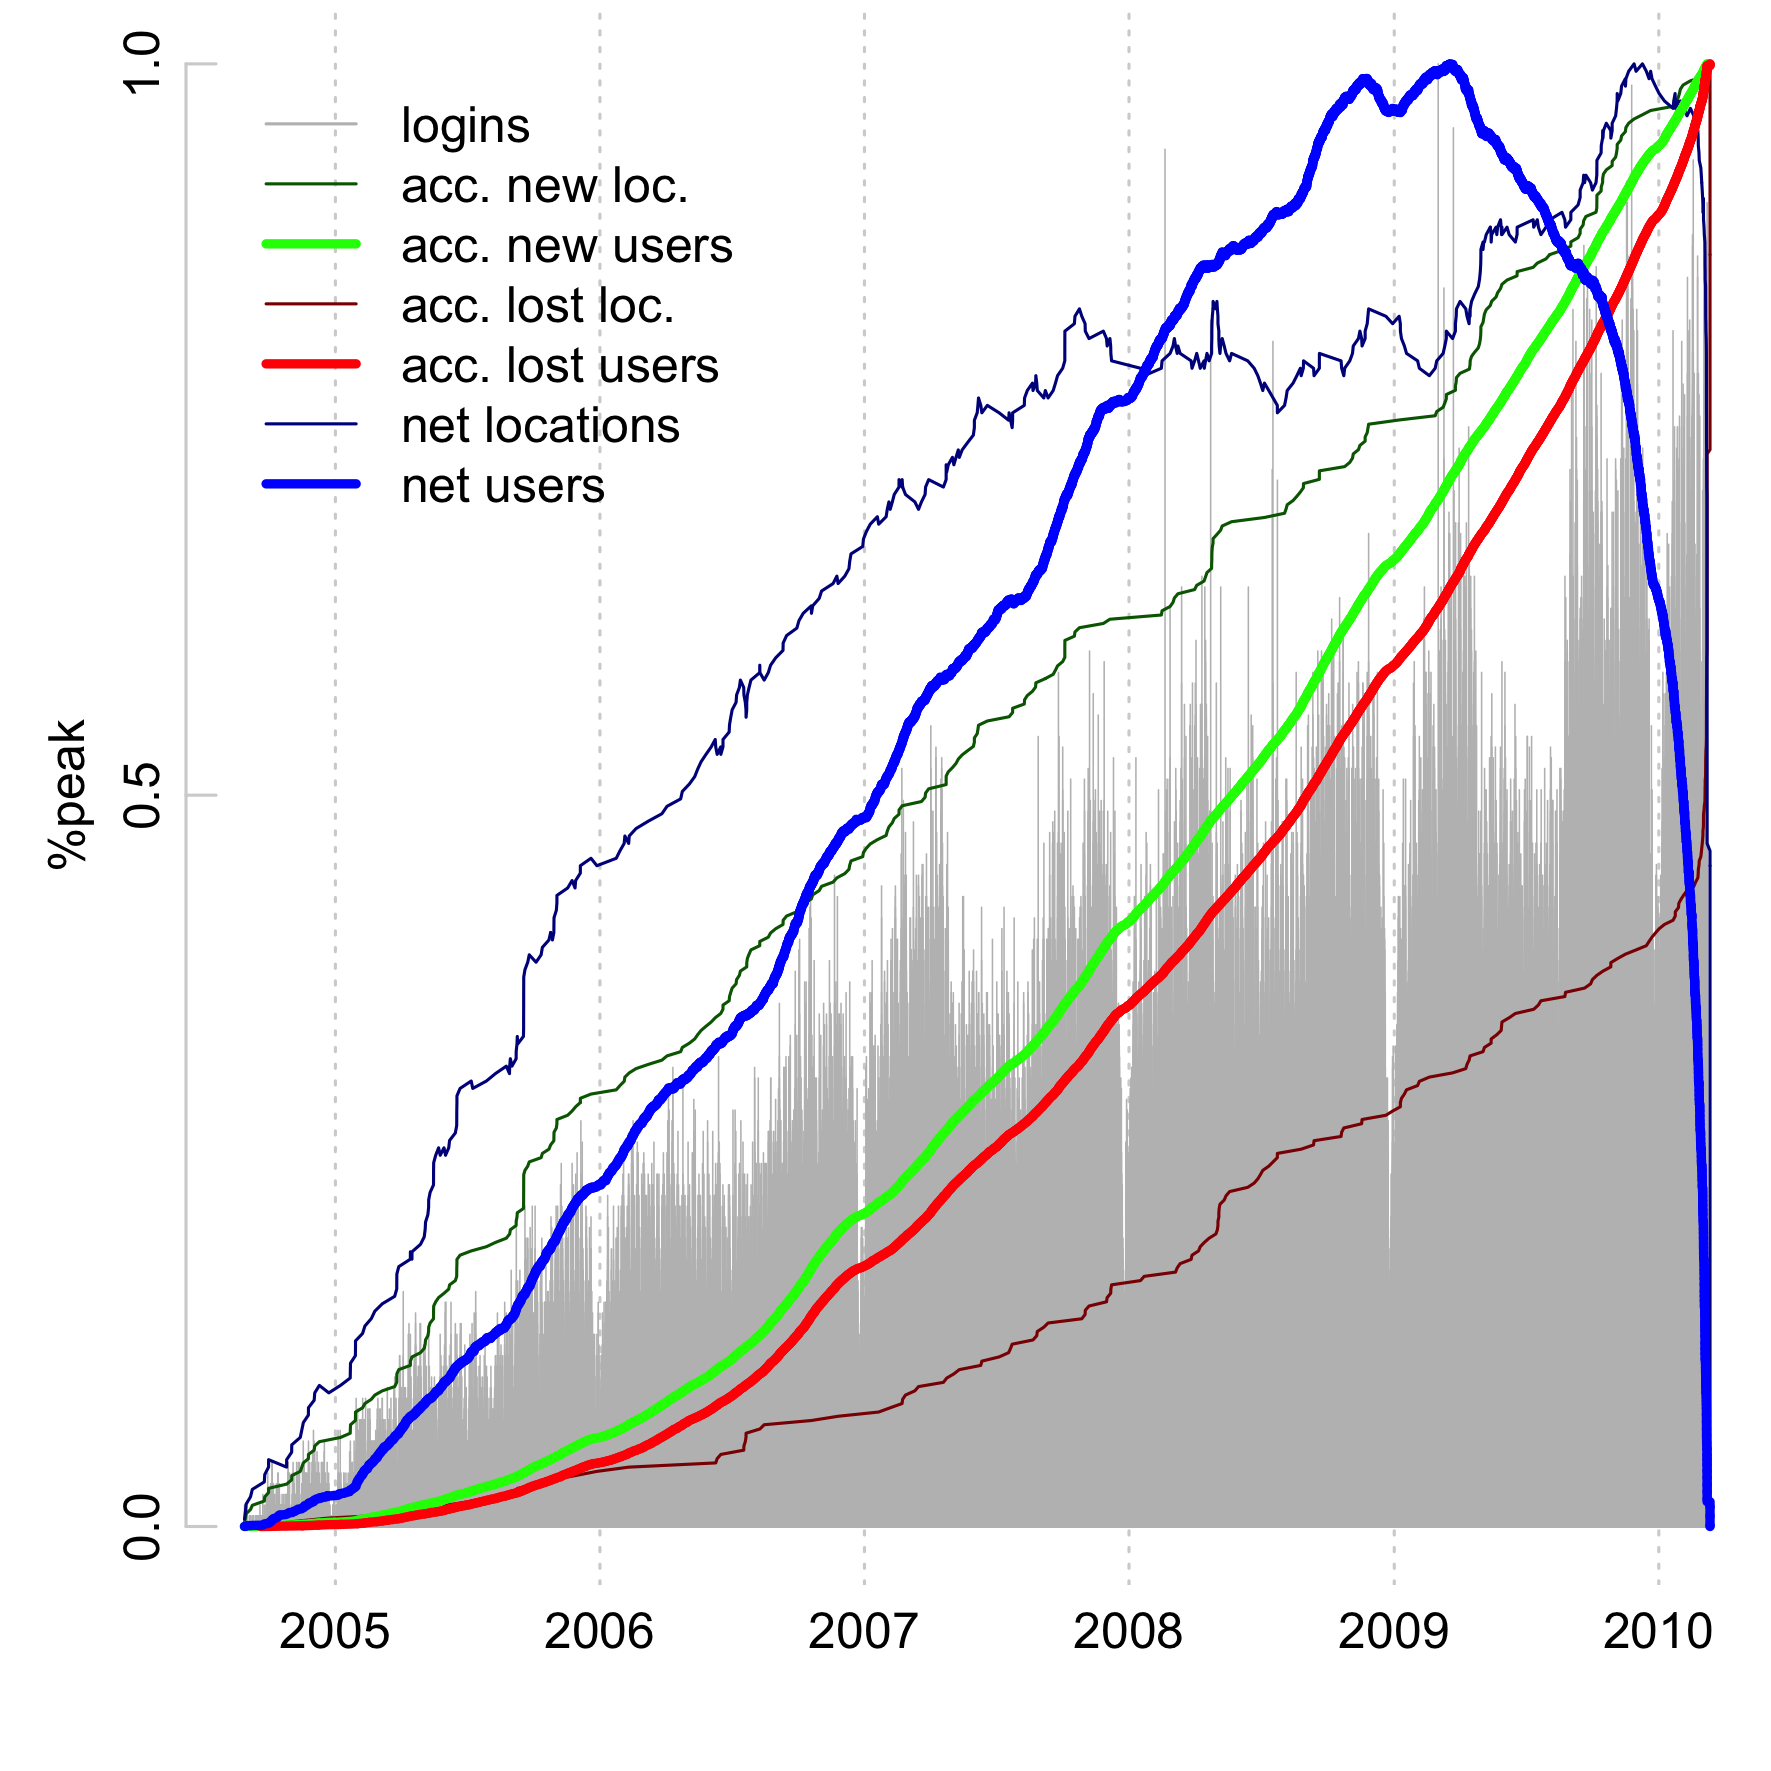
\includegraphics[width=1.0\linewidth]{dataReview.png}
    \end{figure}   
    \end{oneCol}
    \spacer{}
    \begin{oneCol}
    \end{oneCol}
    \spacer{}
    \begin{oneCol}
    \end{oneCol}
    \end{columns}
%    \begin{figure}
%<<plotfig1,fig=TRUE,echo=FALSE>>=
% graph.measure.plotting()
%@
%    
\includegraphics[width=0.8\linewidth]{placeholder.jpg}
%    \caption{The first figure should be a series of comparisons of network measures (e.g., degree distribution) for the totally aggregated network vs averaged values of the network aggregated at different time periods - 1 year, 1 month, 1 week, 1 day.  May also want to do some heat charts of those measures through time, since the averages might hide neat insights like seasonality.  I also think we could use some plots of something approximating edge weights -- like the distribution of edge duration proportion (time edge exists as fraction of interval).}
 %   \end{figure}
    \begin{figure}
    
\includegraphics[width=0.8\linewidth]{placeholder.jpg}
    \caption{This should be the figure showing the simulation results for aggregation on whole network vs having day-by-day networks.  Probably should be two figures, one for final sizes and one for trajectories.  If we have time, multiples of these for some parameter variation.}
    \end{figure}
    
    \end{block}
    \vfill
    \end{threeCol}
    \spacer{}
    \end{columns}
  \end{frame}
  \end{document}
 



% 
% 
% %----------------------------------------------------------------------------------------
% %	ADDITIONAL INFORMATION
% %----------------------------------------------------------------------------------------
% 
% \begin{block}{Additional Information}
% 
% Maecenas ultricies feugiat velit non mattis. Fusce tempus arcu id ligula varius dictum. 
% \begin{itemize}
% \item Curabitur pellentesque dignissim
% \item Eu facilisis est tempus quis
% \item Duis porta consequat lorem
% \end{itemize}
% 
% \end{block}
% 
% %----------------------------------------------------------------------------------------
% %	REFERENCES
% %----------------------------------------------------------------------------------------
% 
% \begin{block}{References}
% 
% \nocite{*} % Insert publications even if they are not cited in the poster
% \small{\bibliographystyle{unsrt}
% \bibliography{sample}\vspace{0.75in}}
% 
% \end{block}
% 
% %----------------------------------------------------------------------------------------
% %	ACKNOWLEDGEMENTS
% %----------------------------------------------------------------------------------------
% 
% \setbeamercolor{block title}{fg=red,bg=white} % Change the block title color
% 
% \begin{block}{Acknowledgements}
% 
% \small{\rmfamily{Thank the data source + ARO grant that's paying for CABP to attend.}} \\
% 
% \end{block}
% 
% %----------------------------------------------------------------------------------------
% %	CONTACT INFORMATION
% %----------------------------------------------------------------------------------------
% 
% \setbeamercolor{block alerted title}{fg=black,bg=norange} % Change the alert block title colors
% \setbeamercolor{block alerted body}{fg=black,bg=white} % Change the alert block body colors
% 
% \begin{alertblock}{Contact Information}
% 
% \begin{itemize}
% \item Web: \href{http://github.com/pearsonca/epidemics-4talk}{http://github.com/pearsonca/epidemics-4talk}
% \item Email: \href{mailto:cap10@ufl.edu}{cap10@ufl.edu}, \href{mailto:thladish@ufl.edu}{thladish@ufl.edu}
% \end{itemize}
% 
% \end{alertblock}
% 
% \begin{center}
% \begin{tabular}{ccc}
% 
\includegraphics[width=0.4\linewidth]{logo.png} & \hfill & 
\includegraphics[width=0.4\linewidth]{logo.png}
% \end{tabular}
% \end{center}
% 
% %----------------------------------------------------------------------------------------
% 
% \end{column} % End of the third column
% 
% \end{columns} % End of all the columns in the poster
% 
% \end{frame} % End of the enclosing frame
% 
% \end{document}
